\chapter{Simulation und Testplanung}
Um das Potentialfeld auch ohne Robotinos zu testen, wird zu Beginn des Projektes mit einer vereinfachten Simulation das Potentialfeld auf Ihre Funktionsf�higkeit gepr�ft. Bei dieser Simulation wird der Robotino als einfache I-Strecke betrachtet. Dabei wird der Ausgang der Strecke auf dem Istpositionsinput gegeben und der berechnete Geschwindigkeitsvektor auf die Strecke gegeben. Des Weiteren werden auf die restlichen Inputs Konstanten gegeben und die Ausgangsdaten in einer Logdatei abgespeichert. Da nach wenigen Versuchen erkennbar ist, dass das Potentialfeld seine Funktion erf�llt, wird im Folgenden mit den Robotinos direkt getestet. Dazu wird zu Beginn der Fertigungsbereich nicht betrachtet und nur ein fest programmiertes Ziel angefahren. Um flexibel Ziele anfahren zu k�nnen und die Schnittstelle mit der Fertigungsplanung zu testen, wird ein UDP-Dummy in Simulink erstellt, mit dem Auftr�ge an den Robotino per UDP in Simulink gesendet werden k�nnen. Dadurch k�nnen mehrere Ziele hintereinander Angefahren werden. Im n�chsten Schritt wird die Schnittstelle mit der Bahnregelung getestet. Dazu werden beide Simulinkmodelle kombiniert und auf den Robotino geladen. Dadurch k�nnen Schnittstellenprobleme zwischen der Bahnregelung und der Bahnplanung fr�hzeitig behoben werden. Da sich im Laufe des Projektes gezeigt hat, dass die Fertigungsplanung den Gesamtsystemtesttermin nicht einhalten kann, wird der UDP-Dummy in Zusammenarbeit mit der Bahnregelung dahingehend erweitert, zufallsgenerierte Auftr�ge zu senden. Im letzten Schritt wird der UDP-Dummy als Fertigungsplanungsersatz erweitert indem sich die Positionen der Werkst�cke gemerkt werden und die zufallsgenerierten Auftr�ge auf ausf�hrbare Auftr�ge gefiltert wird. Zum Ende des Projektes wird zus�tzlich eine Simulation, wie zu Beginn, mit der Erweiterung auf f�nf Robotinos ausgef�hrt, um geringe �nderungen im Programm aufzuzeichnen, da die Aufzeichnung von Daten von mehreren Robotinos unter Simulink-Realtime einige Probleme verursacht. Unter Kapitel \ref{sec:simAusw} wird eine Simulation des Ausweichman�vers dargestellt und unter Kapitel \ref{sec:simWarte} wird das Verhalten beim Anfahren der Wartebereiche gezeigt.

\section{Simulation des Ausweichman�vers}\label{sec:simAusw}
In diesem Abschnitt wird die Simulation des Ausweichman�vers dargestellt. Dazu werden zwei Simulationen miteinander verglichen. In der ersten Simulation, welche in Abbildung \ref{fig:SimulationAusweich} dargestellt ist, werden zwei Robotinos betrachtet. Robotino 1, in Rot dargestellt, f�hrt von der Position [500 1000] zur Station 7, welche sich ganz rechts befindet. Robotino 2, in Blau dargestellt, f�hrt von der Position [4500 1000] zur Station 0, welche sich ganz links befindet. Wie in der Abbildung zu sehen ist, umfahren sich die Robotinos rechts herum.

\begin{figure}
	\centering	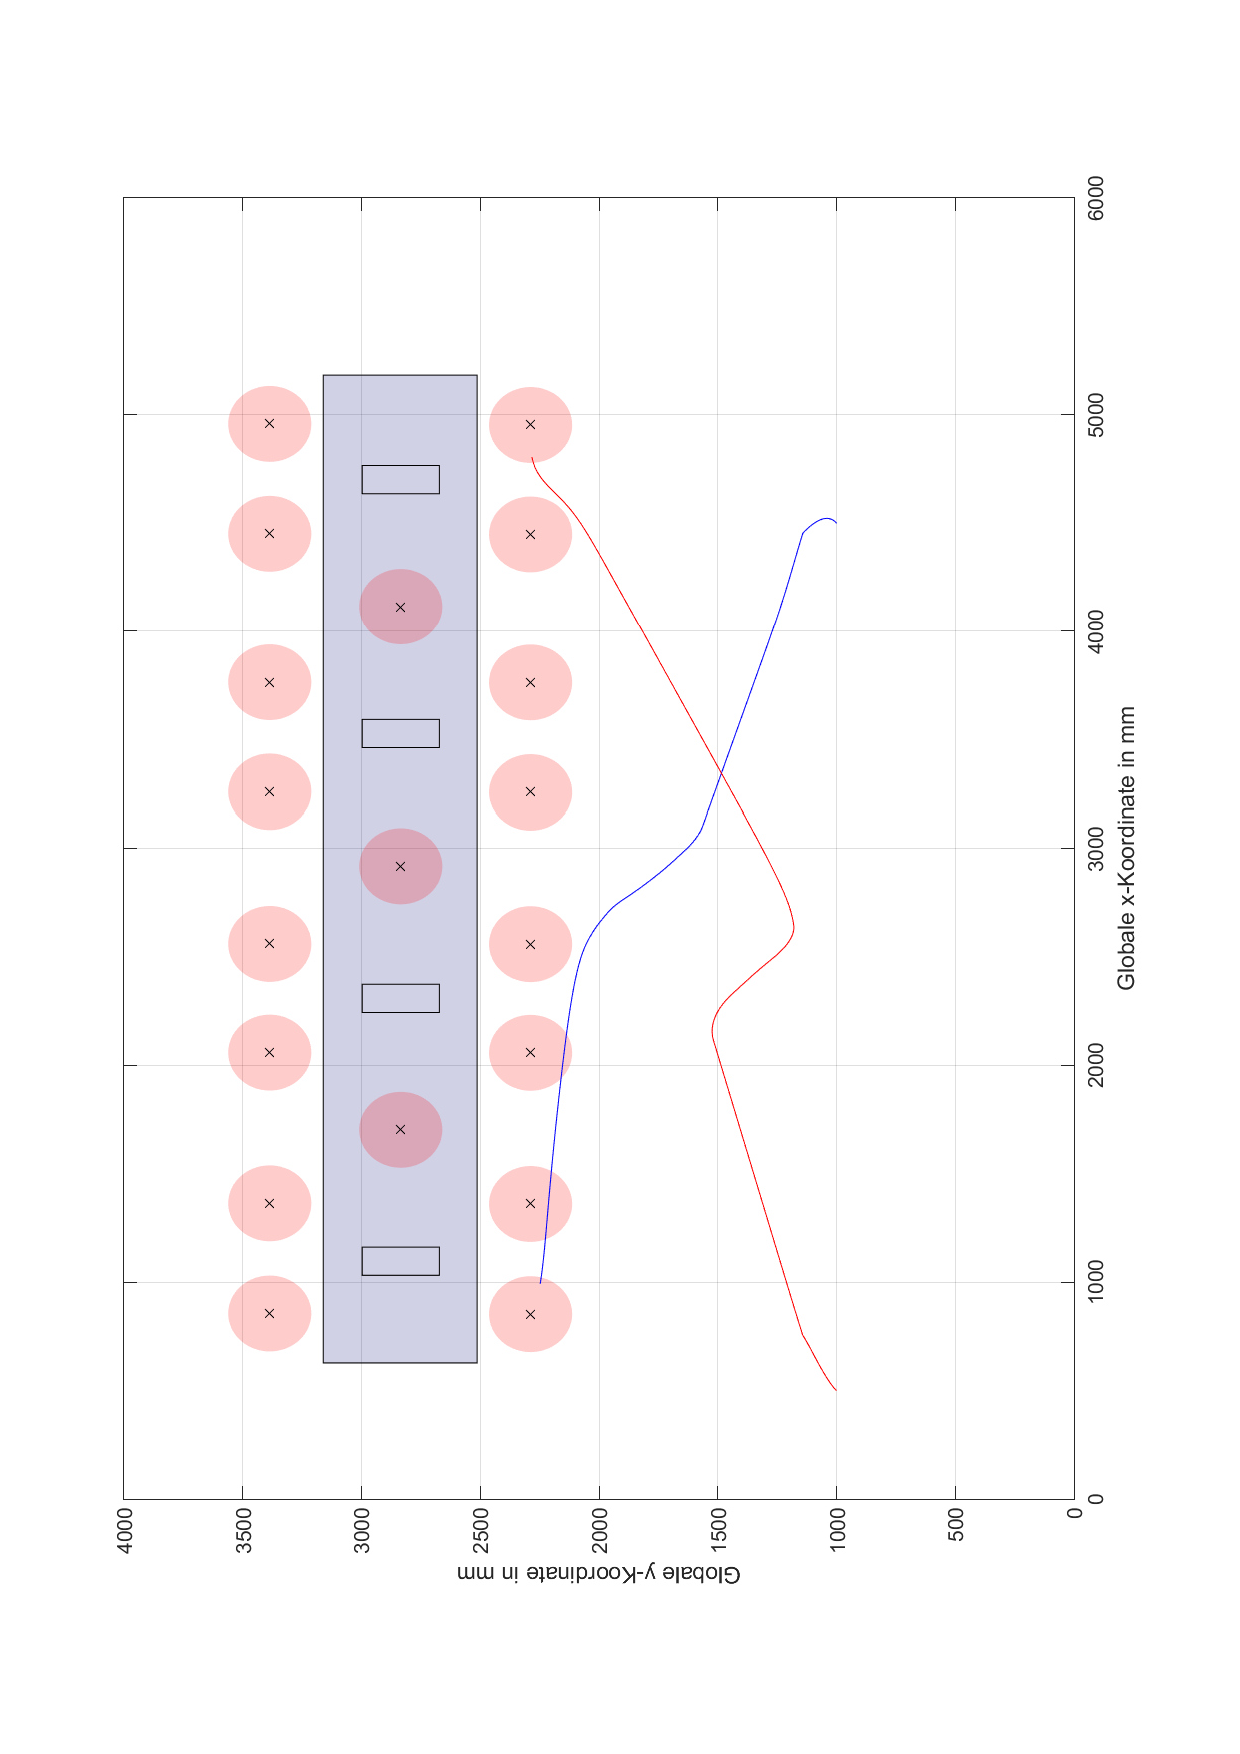
\includegraphics[width=0.8\textwidth,angle=-90]{grafiken/SimulationAusweich.pdf}
	\caption{Simulation mit Ausweichfunktion}
	\label{fig:SimulationAusweich}
\end{figure}

In der zweiten Simulation, welche in Abbildung \ref{fig:SimulationohneAusweich} dargestellt ist, werden die gleichen Robotinos mit der gleichen Start und Zielposition betrachtet. In dieser Simulation wird lediglich die Ausweichfunktion auf Null gesetzt. Wie in der Abbildung zu erkennen ist, kommt es zu einem Absto�verhalten, wodurch die Robotinos stark ausgebremst werden. Wie in den Abbildungen zu erkennen ist, hat die entwickelte Ausweichfunktion eine Verbesserung im Ausweichverhalten verursacht.
 
\begin{figure}
	\centering	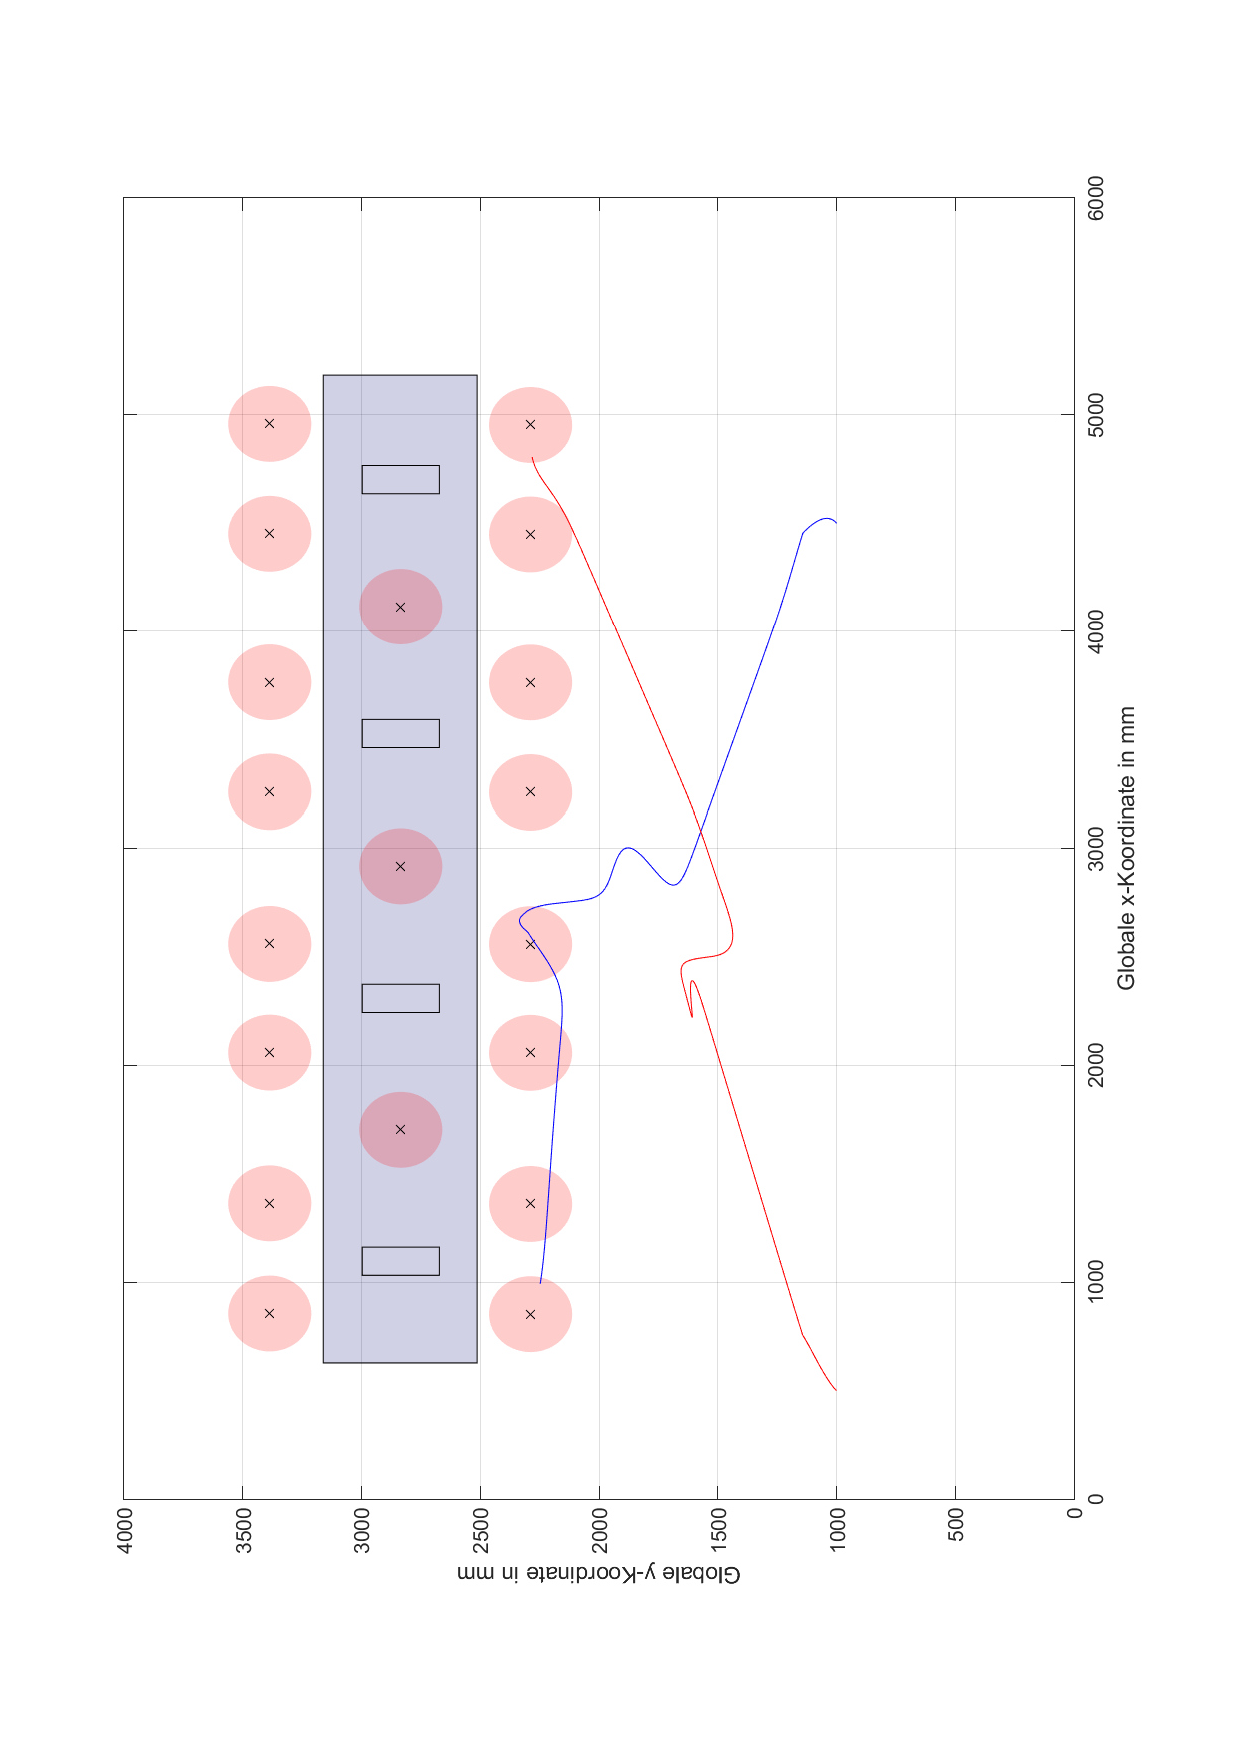
\includegraphics[width=0.8\textwidth,angle=-90]{grafiken/Simulation_ohne_Ausweich}
	\caption{Simulation ohne Ausweichfunktion}
	\label{fig:SimulationohneAusweich}
\end{figure}

\section{Simulation Wartebereiche}\label{sec:simWarte}
In diesem Abschnitt wird eine Simulation der Wartebereiche durchgef�hrt. Dazu werden vier Robotinos im Transportbereich verteilt und sollen das selbe Ziel anfahren. Dadurch kann man das Verhalten der Robotinos bei der Nutzung der Wartepositionen beobachten. In Abbildung \ref{fig:SimulationFIFO} ist das Ergebnis der Simulation dargestellt. Die Zielstation wird in dieser Simulation als 2 definiert. Dabei ist zu erkennen, dass der Robotino mit der Startposition [2000 1000], in Gr�n dargestellt, als erster das Ziel erreicht.\\
Wie am n�chsten Robotino, in Blau dargestellt, zu erkennen ist, wird von seiner Startposition ([1000 500]) erst die Station als Ziel angenommen. Da sich in diesem Moment jedoch der gr�ne Robotino in seiner Fahrtrichtung befindet, wird das unter Kapitel \ref{sec:simAusw} bereits simulierte Ausweichman�ver angewendet, bis der gr�ne Robotino die Station erreicht hat. Dieser Zeitpunkt ist in der Abbildung als schlagartige Richtungs�nderung erkennbar, da in diesem Moment das Ziel auf die erste Warteposition ge�ndert wird. Da sich auf dem Weg zum neuen Ziel keine Robotinos befinden, trifft der blaue Robotino auf der ersten Warteposition als erster ein.\\
Der rote Robotino, mit der Startposition [5000 1000], zeigt bei seiner Fahrt ein �hnliches Verhalten wie der blaue. An der Route kann erkannt werden, dass zuerst gerade auf die Station zugefahren wird. In n�chstem Schritt wird Schlagartig die Richtung auf die erste Warteposition ge�ndert, da der gr�ne Robotino die Station erreicht hat. Die n�chste Auff�lligkeit besteht darin, dass das Ausweichman�ver aufgrund des blauen Robotinos ausgel�st wird. Dadurch wird der Robotino von seiner Ideallinie abgebracht. Da sich der rote Robotino, aufgrund des Ausweichman�vers, beim Eintreffen des blauen Robotinos, auf der ersten Warteposition auf der linken Seite der ersten Warteposition befindet, wird der auf der ersten Warteposition befindliche Robotino umfahren, da sich die Wartepositionen bei geraden Zielstationen nach rechts anh�ngen.\\
Als letztes wird der cyane Robotino betrachtet. Da dieser Robotino �ber den Stationen ([1000 3500]) startet, wird dieser zuerst �ber die F�hrungspotentialfelder zur Hauptfahrzone transportiert. Da sich der gr�ne Robotino beim Wechsel zur Hauptfahrzone bereits in der Station befindet, wird direkt die erste Warteposition als Ziel definiert. Da dieser Robotino auf seiner Route auf den roten Robotino trifft, wird auch hier im Laufe der Route ein Ausweichman�ver erkennbar. Da sich auch dieser Robotino auf die n�chsten Wartepositionen begeben m�chte, sich jedoch der rote Robotino immer vor ihm befindet, stellt sich der cyane Robotino im Laufe der Simulation auf die dritte Warteposition.
\begin{figure}
	\centering	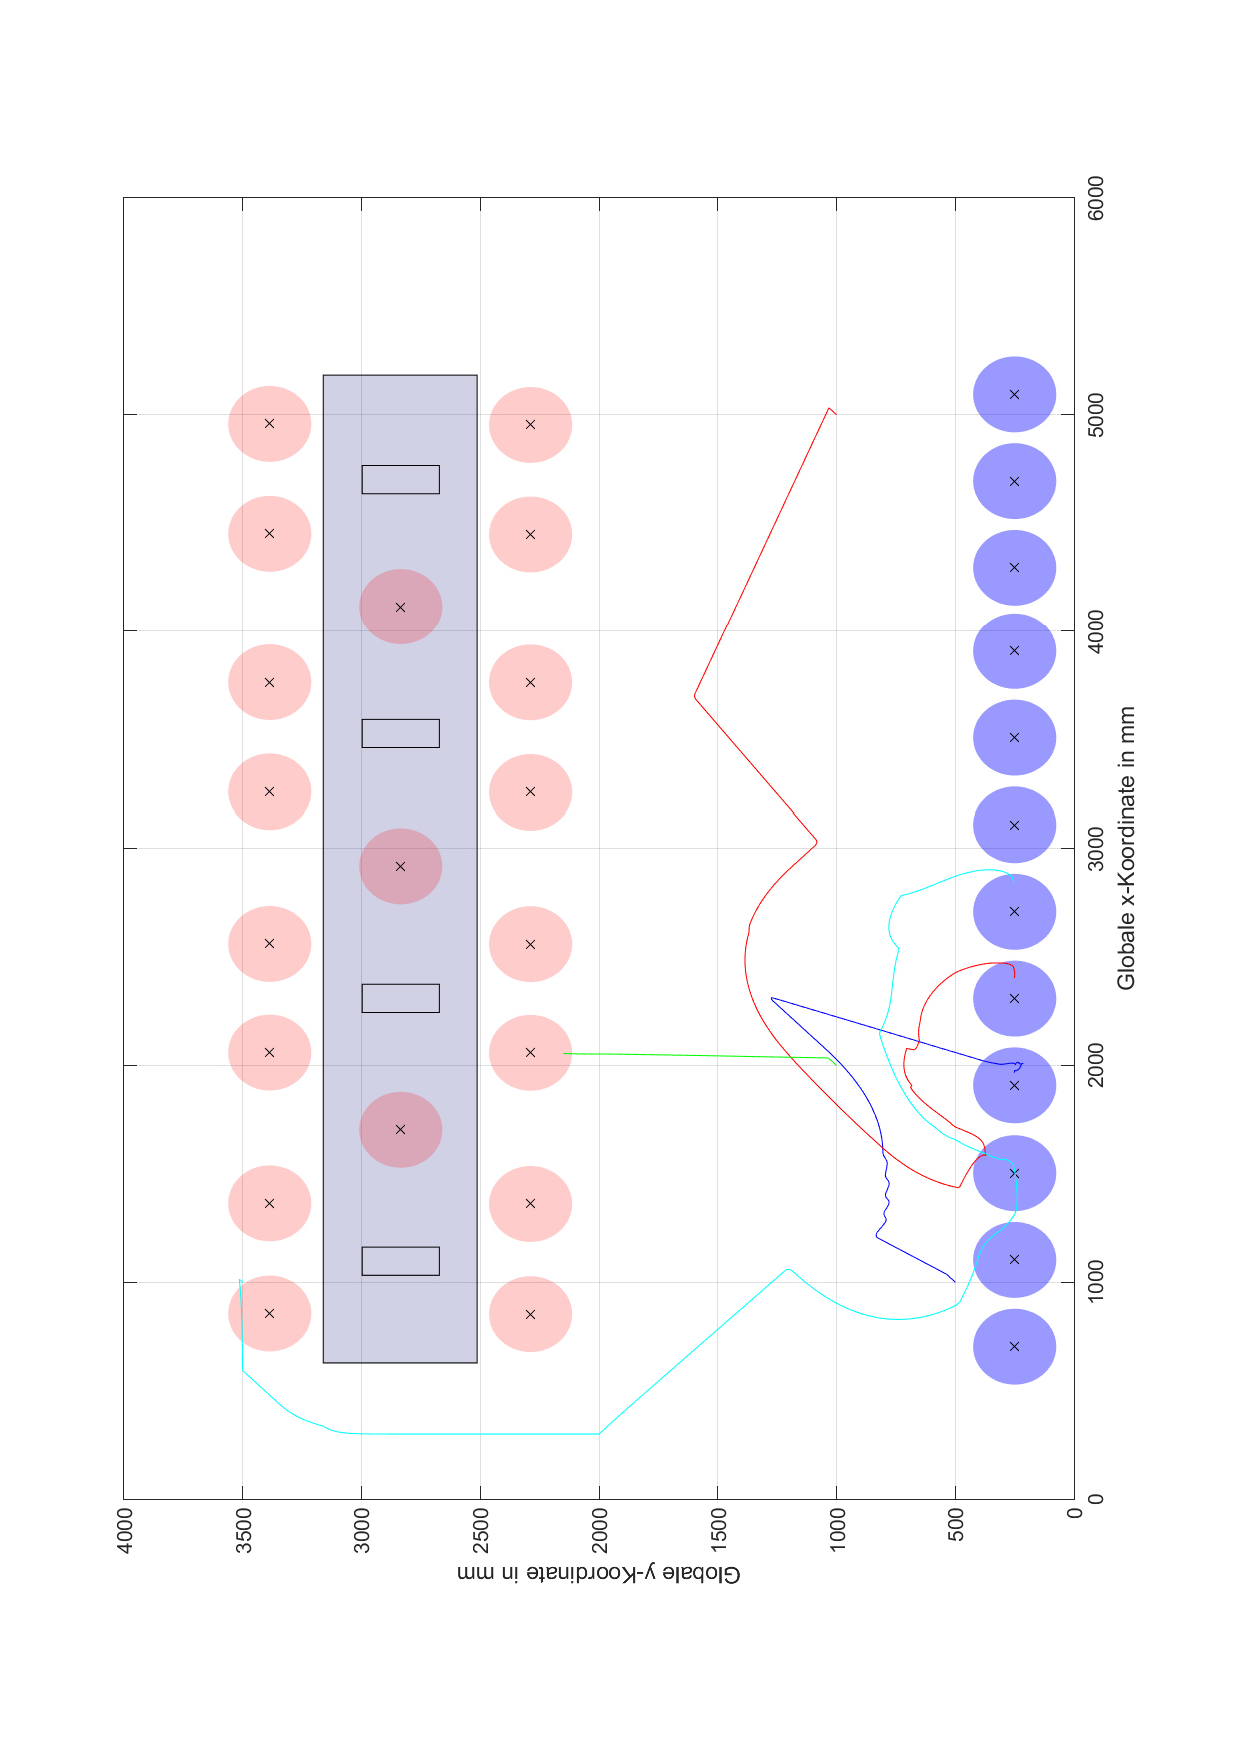
\includegraphics[width=0.8\textwidth,angle=-90]{grafiken/Simulation_FiFo}
	\caption{Simulation der Wartebereiche}
	\label{fig:SimulationFIFO}
\end{figure}